\chapter{Using Compass}
Compass is currently distributed as part of ROSE, and represents one
of many tools that can be built using the ROSE open compiler infrastructure.
The source code of Compass resides in the {\tt ROSE/projects/compass}.
The compass project is currently divided into three subdirectories representing
the compass infrastructure, extensions (checkers), and individual compass-like
tools. As part of building ROSE Compass will be automatically built in the 
compass directory. 

\section{Installation}
\label{usingCompassInstallation}
Please follow
\htmladdnormallink{ROSE Installation
Guide}{http://www.rosecompiler.org/ROSE_InstallationInstructions.pdf} to
configure, make, and make install ROSE. The Compass executable file
(compassMain) will be available from YOUR\_ROSE\_INSTALL\_PATH/bin. compassMain needs to know where to find its own configuration information from two
files:
\begin{itemize}
\item compass\_parameters: configuration information for compass checkers.
A default parameter file is generated in your ROSE build tree:
buildrose/projects/compass/tools/compass/compass\_parameters. You can
save a copy to your home directory for customization. 
\item RULE\_SELECTION: This file lists which checkers to be used. A sample
file is provided in the ROSE source tree:
source/projects/compass/tools/compass/RULE\_SELECTION.in. You can save
it as RULE\_SELECTION in your home directory and flip the $+$ or $-$ sign
before each checker to turn on or off them when running compassMain. This
file is specified as Compass.RuleSelection=/home/youraccount/RULE\_SELECTION
inside of the compass\_parameters file.
\end{itemize}

After preparing compassMain's configuration files, you can set environment variables as follows (assuming using bash
and you configured ROSE using --prefix=/home/youraccount/opt/roseLatest):

\begin{verbatim}
PATH=/home/youraccount/opt/roseLatest/bin:$PATH
export PATH

LD_LIBRARY_PATH=/home/youraccount/opt/roseLatest/lib:$LD_LIBRARY_PATH
export LD_LIBRARY_PATH

export COMPASS_PARAMETERS=/home/youraccount/compass_parameters
\end{verbatim}


\section{Running Compass}

Once properly installed and configured, running compass is a matter of typing {\tt compassMain} 
and handing in a number of options. The {\tt compassMain} program acts just 
like a compiler so it is appropriate to hand it the same options required to 
compile your source file (e.g {\tt -I} directory paths and a source file.  
Compass will figure out the language from the source file suffix.  
Using the {\tt --help} option will provide a more complete list of options 
available to ROSE based tools.  See also the section of this chapter on the 
include/exclude options for path and file names as these will permit the 
output from header files to be tailored.

For example, to test a checker which warns about error-prone pointer
comparison. You can modify RULE\_SELECTION to only turn on
PointerComparison. A test input code (pointerComparisonTest1.C) is provided
in sourcetree/projects/compass/extensions/checkers/pointerComparison. 
\begin{verbatim}
# command line to run compassMain on a source file
compassMain pointerComparisonTest1.C
# output of the command
 Running Prerequisite SgProject
Running checker PointerComparison
PointerComparison: pointerComparisonTest1.C:16.7-19: 
Warning: Error-prone pointer comparison using <,<=,>,or >=
\end{verbatim}

\section{Output from Compass}

   Output from compass can be generated in a number of forms, the default is
ASCII text output of the messages about rule violations with the source code
position in {\it GNU standard source code position format}.  This form can be
used to interact with external tools (e.g. Emacs) to permit alternative
interface to Compass.  Mechanisms available include:

\begin{itemize}
   \item Emacs: \\
         Detecting errors while you type \ref{compassEmacs} and \ref{Compass_Emacs_Screenshot}.

   \item Vim 7: \\
         Compass can work with Vim 7's QuickFix commands to
         highlight source lines with error messages \ref{Compass_VIM7_Screenshot}. 

   \item CompassGUI: \\
         There is also a Compass GUI for reviewing Compass output and interactively
         rerunning compass and sifting through the output while relating them to the source
         code \ref{Compass_GUI}. This work uses the QRose library produced at Imperial College
         London by Gabriel Coutinho, as part of their development of FPGA tools using ROSE.
         QRose is based on the Qt library and provides a wide number of ROSE aware components
         to make the development of GUIs for ROSE based tools easy.  The source code for the 
         Compass GUI is provided, but this work is unfinished (and required the QRose library
         available from Imperial).

   \item ToolGear post-processing: \\
         Output in XML permits the use of ToolGear (LLNL tool available on the web) for
         viewing Compass generated output.  This mechanism is particularly useful for reviewing
         the results of nightly builds (and associated runs of large projects using
         Compass). See figure \ref{Compass_ToolGear_Screenshot}

   \item ASCII output: \\
         Output in ASCII format is of the form shown in \ref{Compass_ASCII_Output}.  This
         form permits the connection to multiple external tools (the Emacs interface reads
         the ASCII output format directly).
 
\end{itemize}


\begin{figure}
\hspace{-0.7in}
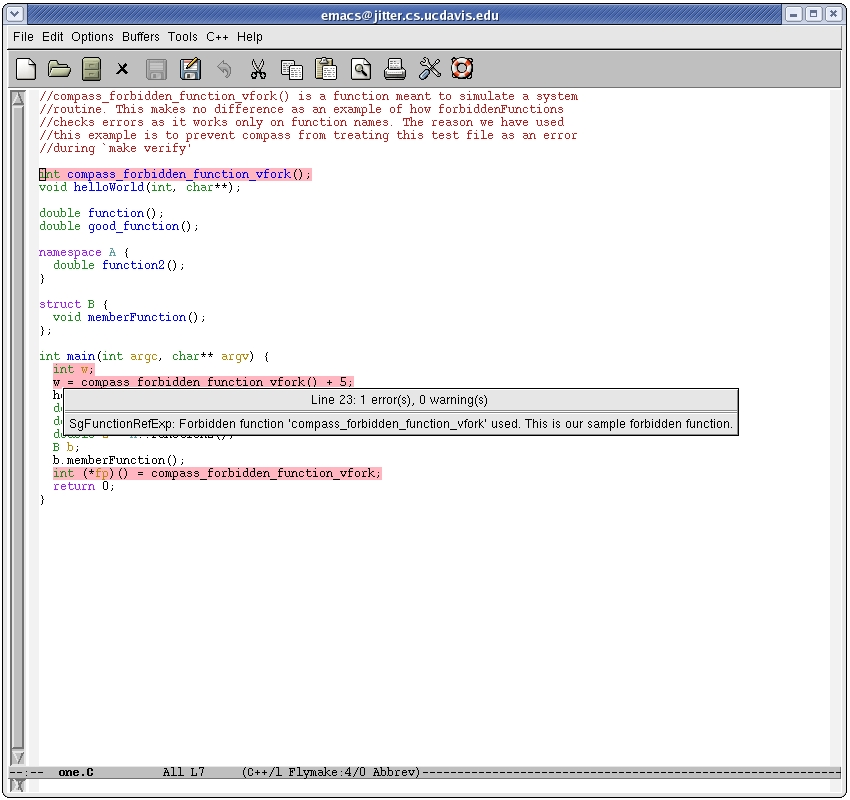
\includegraphics[width=7in]{emacs_screenshot.jpg}
\caption{Compass error messages integrated into Emacs}
\label{Compass_Emacs_Screenshot}
\end{figure}

\begin{figure}
%\center
\hspace{-1.35in}
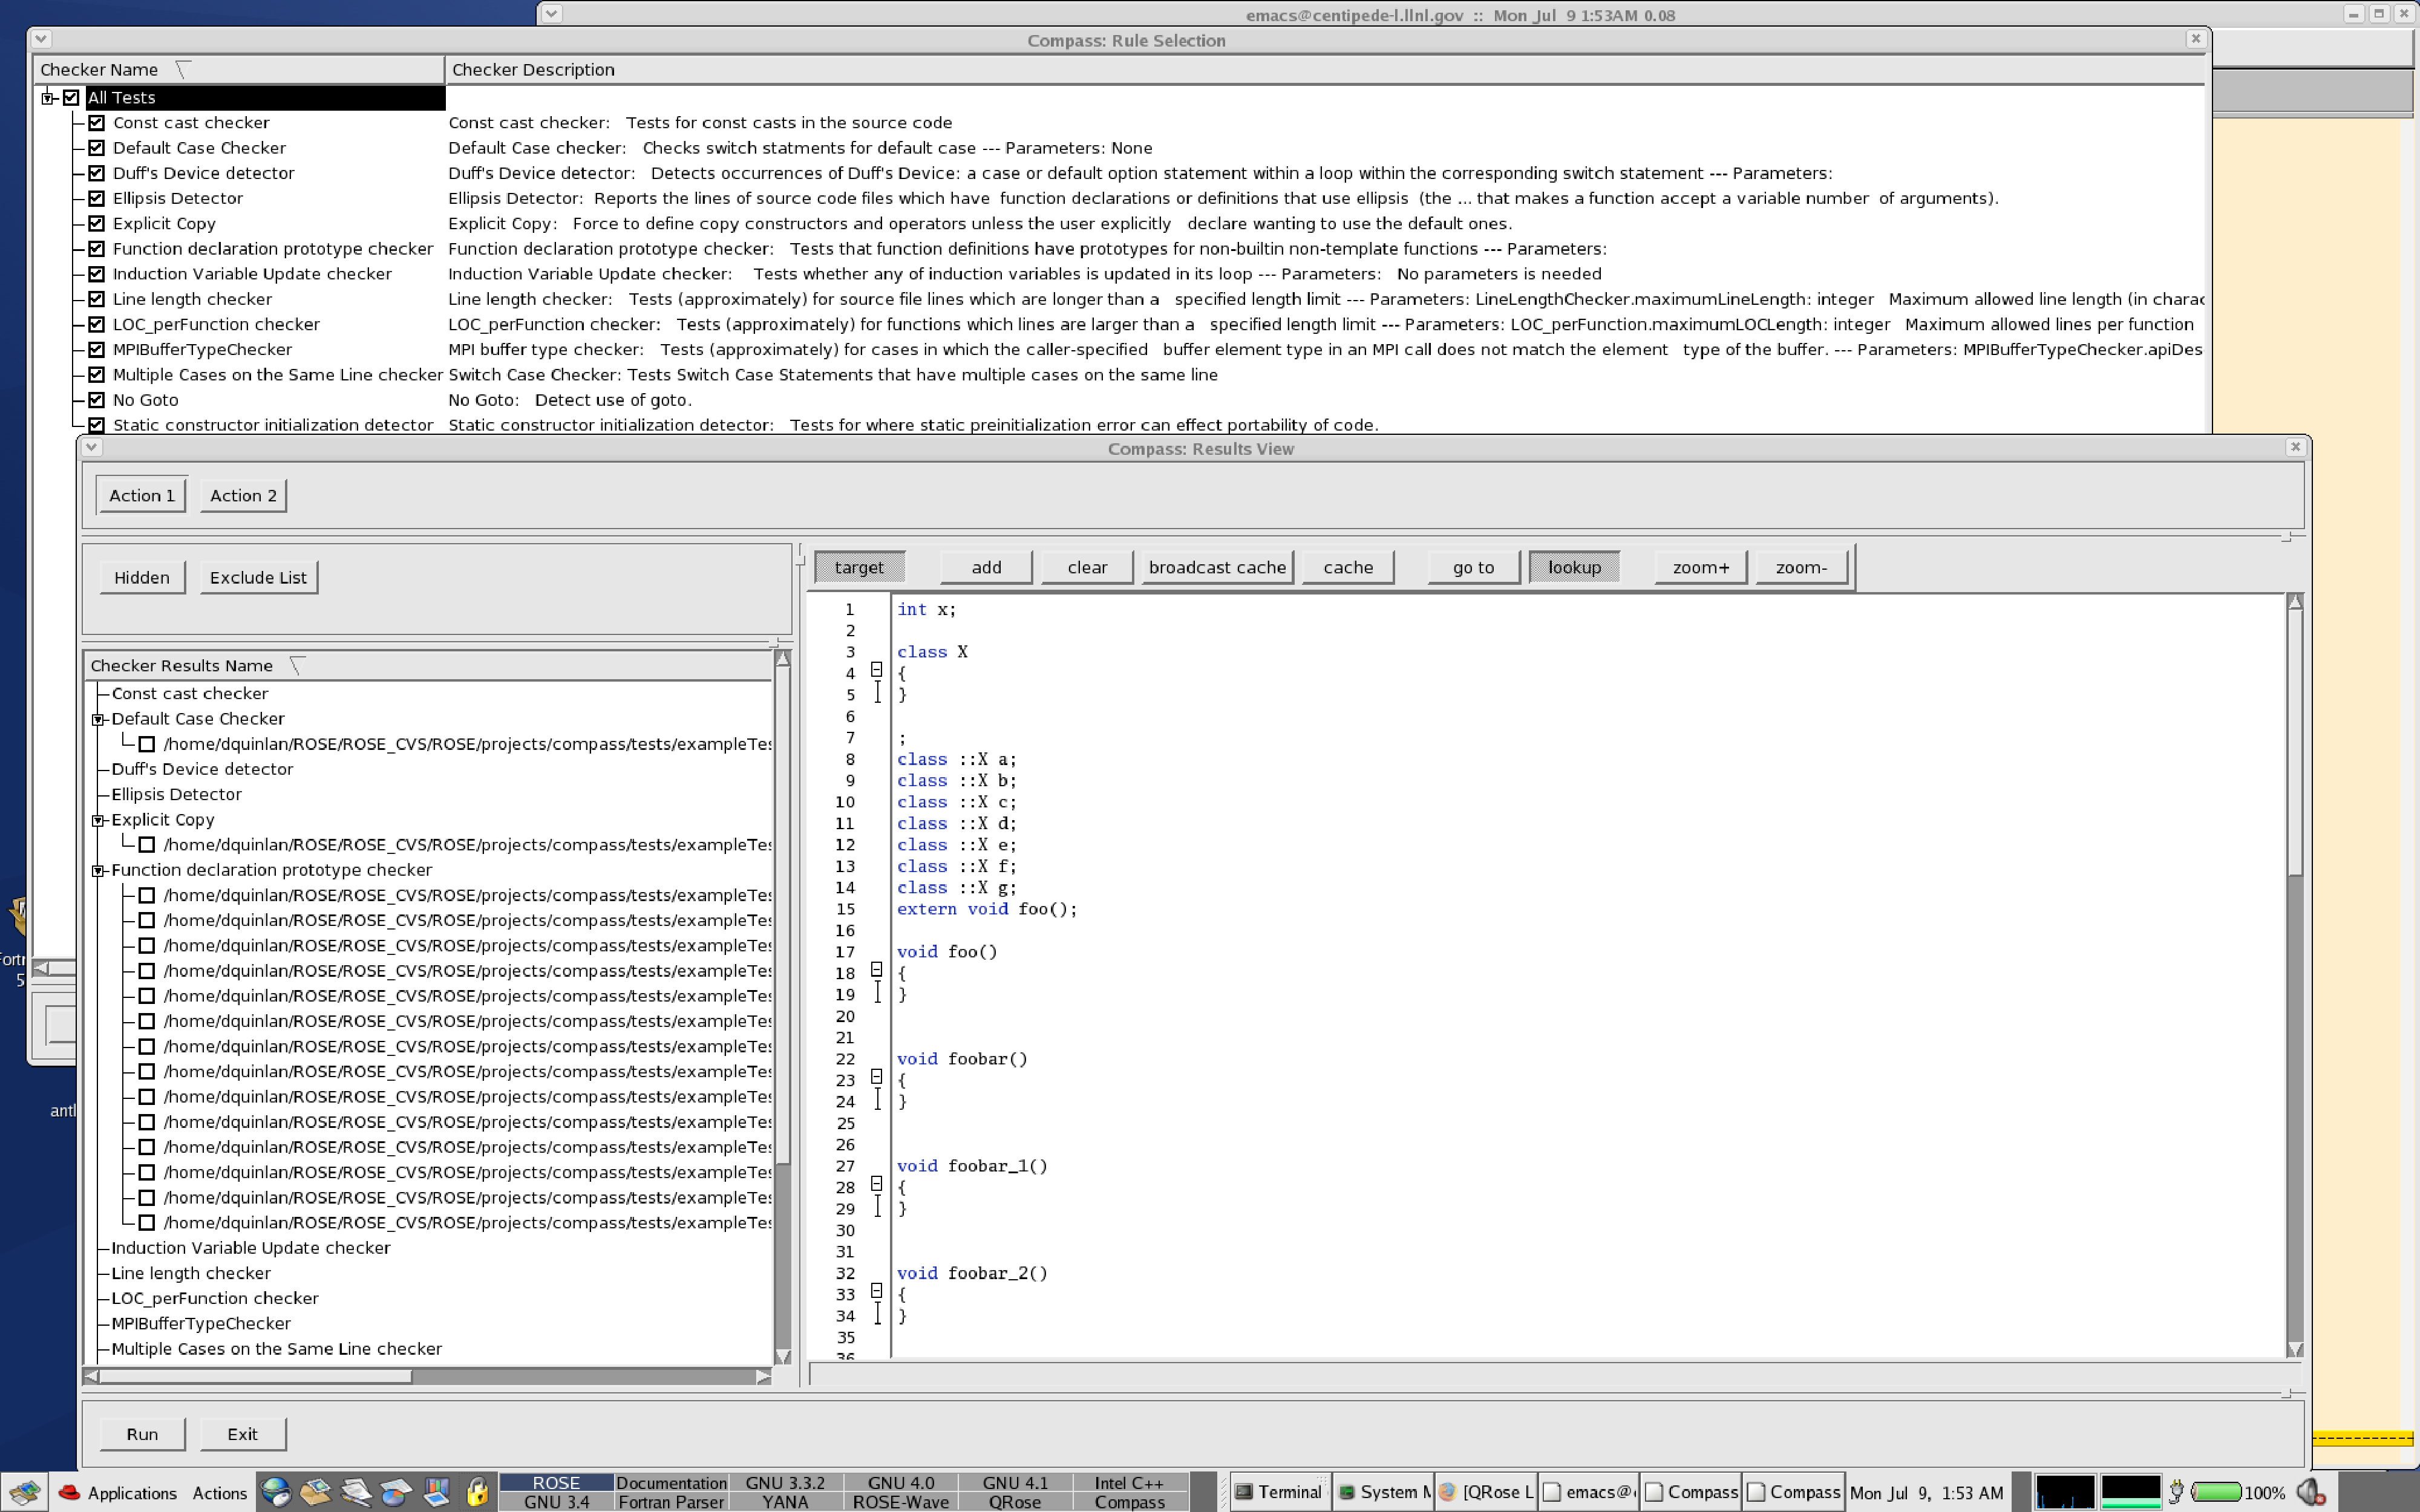
\includegraphics[width=7in]{CompassScreenshot.pdf}
\caption{Compass GUI for interpretation of rule violations}
\label{Compass_GUI}
\end{figure}

\begin{figure}
\hspace{-0.7in}
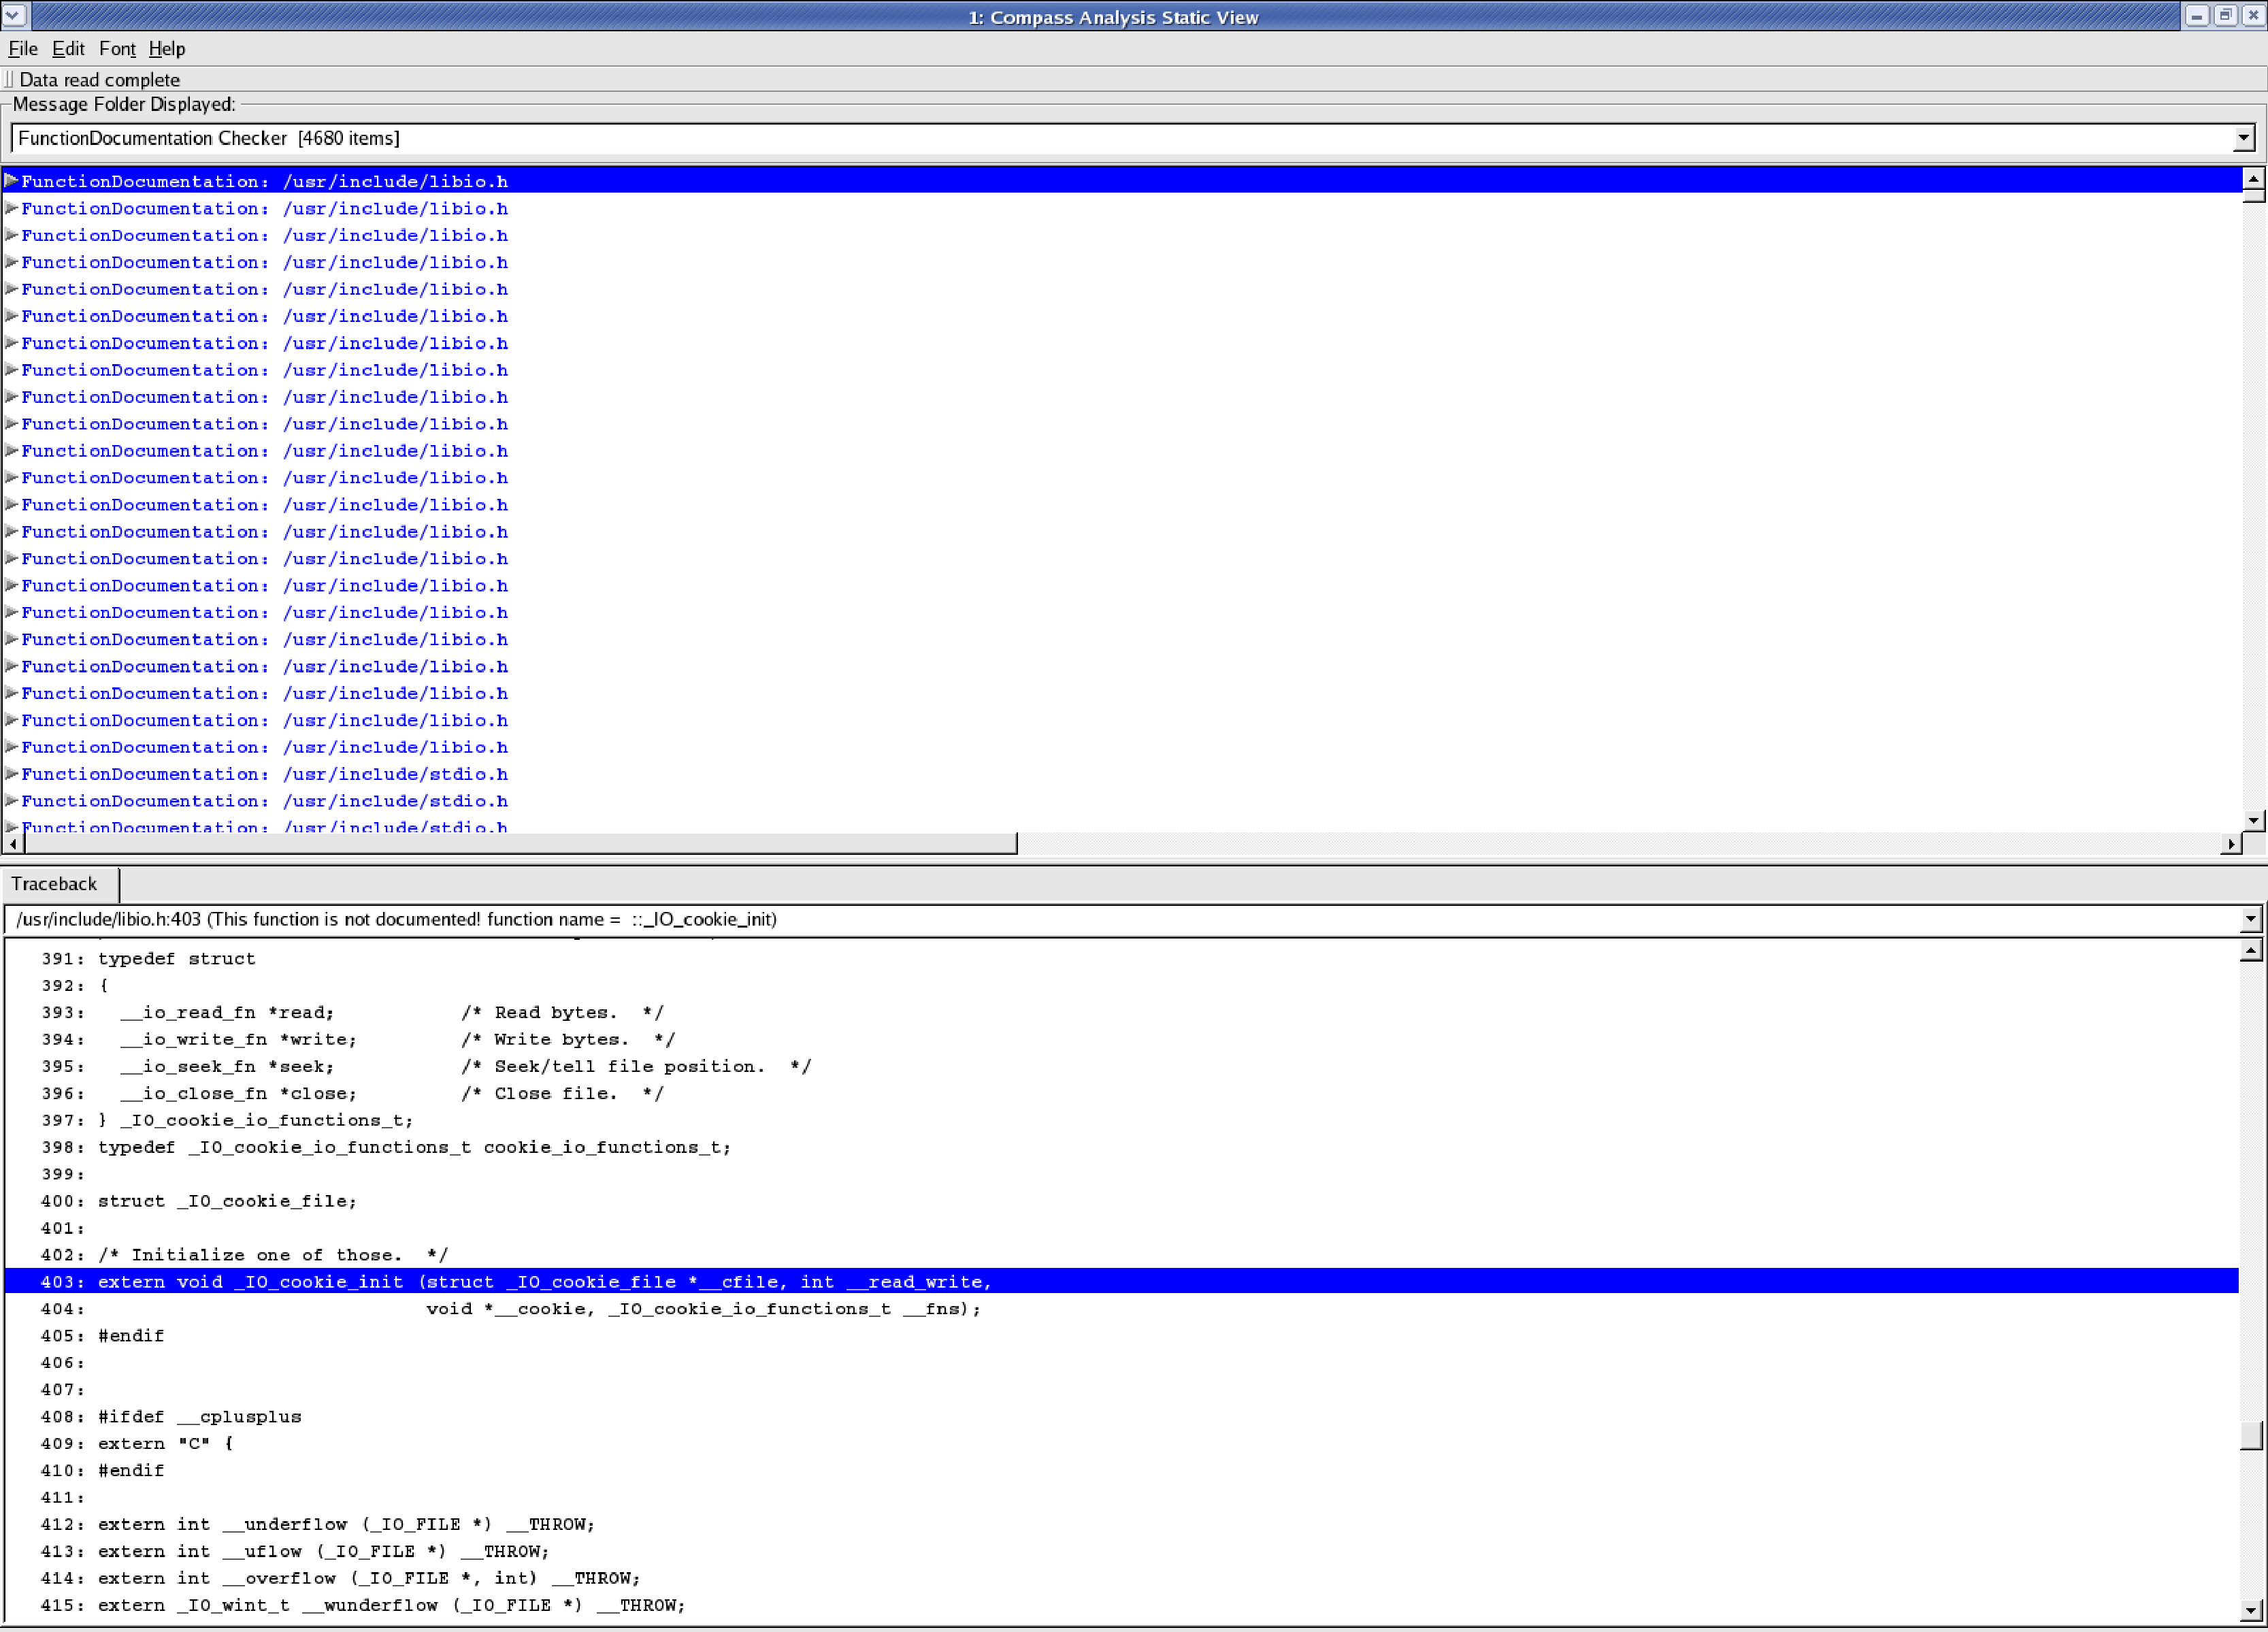
\includegraphics[width=7in]{ToolGear_gui_compass_01.pdf}
\caption{Processing of XML Compass output using ToolGear}
\label{Compass_ToolGear_Screenshot}
\end{figure}

\begin{figure}
{\scriptsize
\begin{verbatim}
LocalizedVariables: /home/ROSE/projects/compass/tests/Cxx_tests/test2006_117.C:30.5: Variable pmNull does not seem to be used.
FunctionDefinitionPrototype: /home/ROSE/projects/compass/tests/Cxx_tests/test2006_123.C:27.1-10: matching function prototype not available
LocPerFunction: /home/ROSE/projects/compass/tests/Cxx_tests/test2006_117.C:23.1-20: This function has too many lines of code :: LOC = 14 > 10
MagicNumber: /home/ROSE/projects/compass/tests/Cxx_tests/test2006_117.C:33.14: Occurrence of integer or floating constant.
MagicNumber: /home/ROSE/projects/compass/tests/Cxx_tests/test2006_117.C:36.14: Occurrence of integer or floating constant.
MagicNumber: /home/ROSE/projects/compass/tests/Cxx_tests/test2006_117.C:37.14: Occurrence of integer or floating constant.
FunctionDocumentation: /home/ROSE/projects/compass/tests/Cxx_tests/test2006_123.C:27.1-10: function is not documented: name =  ::main
FunctionDocumentation: /home/ROSE/projects/compass/tests/Cxx_tests/test2006_123.C:9.10: function is not documented: name =  ::X < int , int , 10 > ::f
FunctionDocumentation: /home/ROSE/projects/compass/tests/Cxx_tests/test2006_123.C:12.10: function is not documented: name =  ::X < int , int * , 5 > ::f
FunctionDocumentation: /home/ROSE/projects/compass/tests/Cxx_tests/test2006_123.C:16.10: function is not documented: name =  ::X < int * , float , 10 > ::f
\end{verbatim}
}
\caption{Example of ASCII output from Compass. }
\label{Compass_ASCII_Output}
\end{figure}



\subsection{Using Compass With Emacs}

\label{compass::emacs}

Compass as a checker is most useful when the user is notified as early as possible
when he violates a desired software property. Although for many purposes it is
sufficient to run Compass separately; it is possible to use compass
seamlessly when developing in emacs. By using an emacs extension called {\em flymake} together
with Compass erroneous lines can be highlighted while programming, and the relevant error messages displayed 
in a dialog. Syntax errors from ROSE will be displayed as well, see figure \ref{Compass_Emacs_Screenshot}.

Much thanks for David Svoboda at CERT at CMU for first configuring Flymake to work with
Compass and demonstrating the idea.  It has provided a great way to check code using
compass and its use in Emacs has stimulate a number of ideas that have made their way
back into Compass.

\subsubsection{Emacs .emacs Code Requirement}

   Figure \ref{compassEmacs} shows the code that is required to be added to the {\tt .emacs}
file.  A copy of this code is available in the compass source directory in the file
{\tt emacs\_compass\_config.el}.

\begin{figure}
{\scriptsize
\begin{verbatim}
; New Compass support for Emacs using version 22 of Emacs and Flymake.
; Comment out these two lines to use older version of emacs.
(require 'flymake)
(setq flymake-allowed-file-name-masks (cons '(".+\\.C\\'" flymake-simple-make-init flymake-simple-cleanup flymake-get-real-file-name) flymake-allowed-file-name-masks))


(defun flymake-master-make-header-init ()
  (flymake-master-make-init 'flymake-get-include-dirs
			    '("\\.C\\'" "\\.c\\'")
			    "[ \t]*#[ \t]*include[ \t]*\"\\([[:word:]0-9/\\_.]*%s\\)\""))

(add-hook 'find-file-hook 'flymake-find-file-hook)

(setq flymake-log-level 3)
(setq flymake-no-changes-timeout 0.5)

(defcustom rose-source-tree "/home/dquinlan/ROSE/NEW_ROSE/" "Location of top of ROSE source tree")
(defcustom rose-build-tree "/home/dquinlan/ROSE/ROSE_CompileTree/LINUX-64bit-3.4.6/" "Location of top of ROSE build tree")
(defun add-buildfile-dir-for-rose ()
  (let ((source-dir-name (file-name-directory buffer-file-name)))
    ;(message "%S" `(source dir ,source-dir-name))
    (if
      ; (string-equal rose-source-tree (substring source-dir-name 0 (length rose-source-tree)))
        (string-equal rose-source-tree (substring source-dir-name 0 (min (length source-dir-name) (length rose-source-tree))))
        (let ((buildfile-dir (concat "../../../../../../../../../../../../../../../../../../../" rose-build-tree "/" (substring source-dir-name (length rose-source-tree)))))
        ; (message "%S" `(buildfile-dir ,buildfile-dir))
        ; (set-variable 'flymake-buildfile-dirs (cons buildfile-dir flymake-buildfile-dirs) 'local))
          (set-variable 'flymake-buildfile-dirs (append (mapcar (lambda (dir) (concat buildfile-dir "/" dir)) flymake-buildfile-dirs) flymake-buildfile-dirs) 'local))
      (progn
        ;(message "%S" `(bad-prefix))
        source-dir-name))))
(defun set-rose-source-dir (dir) "Set the top of the ROSE source tree to use with Flymake" (interactive "DThe top of the ROSE source tree: \n")
  (setq rose-source-tree dir 'local)
  (add-buildfile-dir-for-rose))
(defun set-rose-build-dir (dir) "Set the top of the ROSE build tree to use with Flymake" (interactive "DThe top of the ROSE build tree: \n")
  (setq rose-build-tree dir 'local)
  (add-buildfile-dir-for-rose))

(add-hook 'find-file-hook 'add-buildfile-dir-for-rose)

;(list "make"
;;  (list "-s" "-C" "/home/dquinlan/ROSE/NEW_ROSE/developersScratchSpace/Dan/EmacsCompass_tests/"
;    (list "-s"
;   (list "-s -C" "`pwd | sed 's@^/home/dquinlan/ROSE/NEW_ROSE/@/home/dquinlan/ROSE/ROSE_CompileTree/LINUX-64bit-3.4.6/@'`"
;	   (concat "CHK_SOURCES=" source)
;	     "SYNTAX_CHECK_MODE=1"
;		   "check-syntax"))

(global-set-key [f3] 'flymake-display-err-menu-for-current-line)
(global-set-key [f4] 'flymake-goto-next-error)

\end{verbatim}
}
\caption{Addition to .emacs when integrating Compass into emacs. }
\label{compassEmacs}
\end{figure}

\subsubsection{Emacs Version Requirement}

Emacs version 22 or newer is required to take advantage of the emacs integration of
Compass. Before using Compass a 3 step process must be followed:
\begin{itemize}
   \item Add the text in figure \ref{compassEmacs} (in \\*{\tt ROSE/AUG0508/ROSE/projects/compass/tools/compass/emacs\_compass\_config.el}) to .emacs
   \item Change /path/to/makefile in figure \ref{compassEmacs} to the path to the project you are editing in Compass
   \item Add a 'check-syntax' rule to the makefile of the project that you are working
   on in Compass. This rule should compile all the files you want Compass to check 
   or all files that you are editing with Compass as the compiler.
\end{itemize}

Figure \ref{compassEmacs} shows the needed changes in .emacs for integrating
Compass. The last two lines are the most interesting lines since they introduce two
shortkeys. [f3] can be clicked in order to display all errors for the current line while
[f4] will move the cursor to the next error. 

A short explanation of the code in figure \ref{compassEmacs} is that the first line will require 
the flymake extension to be available upon
loading emacs while the second line will load the find-file-hook and flymake-find-file-hook
functions. The "setq" sections that follows runs Compass for all files that are being edited
that has the c and C extensions. The ``list'' section tells flymake to execute the check-syntax
rule in the makefile. 

\subsubsection{Example check-syntax rule}


\begin{figure}
\begin{verbatim}
one: inc.h one.C
        g++ -c one.C
\end{verbatim}
\caption{Example makefile before the Compass addition  }
\label{beforeProjectCheckRule}
\end{figure}


\begin{figure}
\begin{verbatim}
one: inc.h one.C
        g++ -c one.C
		
check-syntax: inc.h one.C
        /path/to/compass/executable/compassMain -c one.C
\end{verbatim}
\caption{Example makefile after addition to support integration of compass  }
\label{projectCheckRule}
\end{figure}


Figure \ref{beforeProjectCheckRule} shows an example makefile that compiles a file
"one.C" using g++. If "one.C" is edited using emacs the addition of the "check-syntax"
rule is needed, as shown in figure \ref{projectCheckRule}.

\subsection {Using Compass With Vim}
%--------------------------------------------
Compass can be used with Vim 7's QuickFix commands to display warning
messages and highlight the source lines in question. A compass compiler
plugin (compass.vim as shown in Figure \ref{compassVim7})  has
been provided for Vim to parse the warning messages outputted by Compass.

Steps to make Compass work with Vim 7
\begin{itemize}
\item Save compass.vim into ~.vim/compiler.  Create the target directory if it
does not exist.
\item Download errormarker.vim from
http://www.vim.org/scripts/script.php?script\_id=1861 and save it
into .vim/plugin . Again, create the target directory first when it does not
exist.
\item Change your Makefile to use an installed compassMain as the compiler
to compile your code.
\item Use quickfix features of Vim 7 as documented at
http://vimdoc.sourceforge.net/htmldoc/quickfix.html. Some frequently used
commands are:
  \begin{itemize}
   \item Specifying the compass plugin to use by typing a command :compiler compass
   \item Open your source code using gvim and set the compiler to Compass by
   \item Compile you code using compassMain, type :make
   \item Display current message, type :cc
   \item Display all messages, type :clist
   \item Jump to next message, type :cnext
  \end{itemize}
\end{itemize}
%-------------------------------
\begin{figure}[!htp]
{\scriptsize
\begin{verbatim}
" Vim compiler file
" Compiler:     ROSE Compass 0.9.2a
" Maintainer:   Chunhua Liao <youraccount@llnl.gov>
" Last Change:  2008 Apr. 3
"
if exists("current_compiler")
  finish
endif
let current_compiler = "compass"

if exists(":CompilerSet") != 2          " older Vim always used :setlocal
  command -nargs=* CompilerSet setlocal <args>
endif

" single line warning
" multiple line warning, %W, %C continue line %Z end of multiple line
CompilerSet errorformat=%s:\ %f:%l%.%c:\ %m,
         \%s:\ %f:%l%.%c-%*\\d:\ %m,
         \%s:\ %f:%l%.%c-%*\\d%.%*\\d:\ %m,
         \\\"%f\"\\,\ line\ %l%*\\D%c%*[^\ ]\ %m
"some notes about the error/warning message format
"Official guide: http://vimdoc.sourceforge.net/htmldoc/quickfix.html#error-file-format
" Each new rule start with a leading \ unless it is the first rule in the
" first line
"  %f: filename %l: line number %c: column number, only one is permitted %m
" actual error/warning message \ :matching a space
"  %*\\d: matching any number

\end{verbatim}
}
\caption{A compiler plugin for Vim 7 compass.vim}
\label{compassVim7}
\end{figure}
%-------------------------------
Figure ~\ref{Compass_VIM7_Screenshot} shows an example of Compass error
messages integrated into Vim 7.
\begin{figure}[!htp]
%\centering
\hspace{-0.7in}
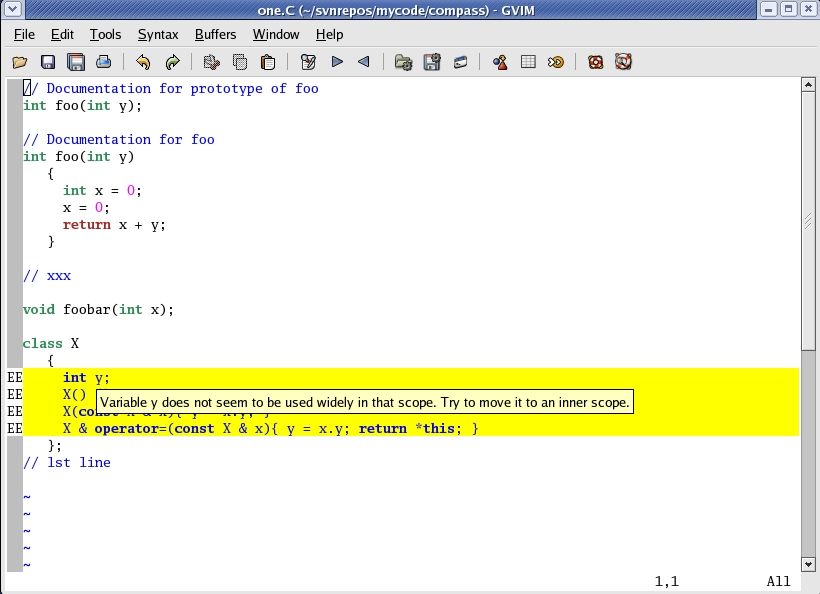
\includegraphics[width=7in]{compass_vim7.jpg}
%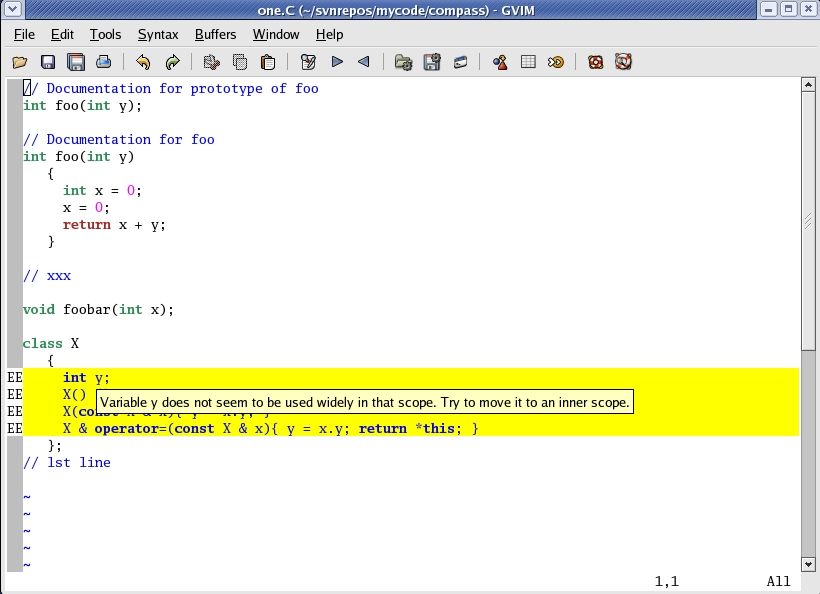
\includegraphics[width=0.7\textwidth]{compass_vim7.jpg}
\caption{Compass error messages integrated into Vim 7}
\label{Compass_VIM7_Screenshot}
\end{figure}


\section{Including/Excluding Checkers in the Compass Build Process}
\label{CompassBuildProcess}

   This section describes how to select which of the checkers to integrate 
into Compass out of all the checkers available in source form in the Compass 
source directory. For security reasons Compass uses this static build process 
since it is a central goal of Compass that it should run as a trusted part of 
a project's build process. If the integration of checkers had been automatic 
through a dynamic plugin mechanism it would be hard to ensure that the dynamic 
list of checkers was secure, but for a static list of trusted checkers this is 
possible.

The file ROSE\_SOURCE\_DIR/projects/compass/tools/compass/CHECKER\_LIST is used to control which checkers are selected to
be compiled into compassMain. It can use the `\#' comment delimiter at the beginning of
any checker name to remove that checker from compilation. The hash mark may
only appear at the beginning of the line. The compass\_submission\_setup.sh
script must be run again with the ``regenerate'' option if any checkers are
commented out. 
{\bf Note that no space is permitted between the `\#' and the name
of the checker.}

Usually the CHECKER\_LIST is only modified when a user or developer wants to 
add a new checker or select a subset of trusted checkers.  Checkers can be
commented out using a {\tt \#}, no space is allowed between the {\tt \#} 
and the checker name.

\section{Including/Excluding Checkers During Compass Execution}
\label{ruleselection}

   This section describes how to execute a subset of the checkers provided in the build
process (see section \ref{CompassBuildProcess}). This process is significantly more
interactive than defining what checkers to include in the Compass build process.
Since it is not unheard of that rules implemented by different checkers can be  
mutually exclusive or even contradicting this mechanism is essential for selecting the
subset of checkers that are interesting for a specific program that is checked.
Separate projects of developers could easily have their own RULE\_SELECTION file
to permit high levels of customization in the use of a Compass tool containing
a large number of checkers (e.g. for different languages).

   When used with the Emacs interface this provides a simple way to turn on and off
specific checkers by editing a single file (RULE\_SELECTION).  The name of this
file is specified in the {\tt compass\_parameters} file, this name may be changed.
The directories searched are: current directory, user home directory, and Compass
source tree (respectively). \fixme{The current implementation may not
support all of the mentioned search paths.}

\begin{verbatim}
   Compass.RuleSelection=/path/to/your/RULE_SELECTION
\end{verbatim}

In order to select a checker to run the user must:
\begin{itemize}
   \item Add a line '-:$<$name of checker$>$' in a file called RULE\_SELECTION. 
   \item If a line  '-:$<$name of checker$>$' already exist the '-' can be modified into
a '+' to enable the checker or into a '-' to disable a checker.
\end{itemize}
It is required that every checker integrated into the Compass build is mentioned in
the RULE\_SELECTION.


\section{Including/Excluding Paths and Filenames with Compass}

    Compass permits paths and filenames to be specified for inclusion/exclusion
in reporting checker rule violations.  Run {\tt compassMain --help} to see
the commandline options.  Numerous other commandline options provided for all
tools build using ROSE may also be relevant.



\section{Checking Security Properties of Checkers}
\label{sec:compass_verify}

    Compass is designed for extensibility while providing the security for
the codes being checked.  To support this Compass provides a simple
mechanism for verifying specific properties of the checkers used in Compass.
Compass implements a specific small number of checkers that are used for checking
the checkers in Compass.  The directory compassVerify contains the implementation
of this subset of Compass that is used on itself.  These checkers may not
be modified and in the future MD-5 checksums will be provided to ensure the
integrity of this subset of Compass.  To verify the compass checkers run:
\begin{itemize}
   \item {\tt make verify} \\
        This makefile rule runs the compassVerify/compassMain on all the source files in
    all the checkers directories in Compass.  Because it runs compass on so
    many separate
    files this step can take a long time.
   \item Or {\tt make oneBigVerify} \\
        The makefile rule runs the compassVerify/compassMain on a single generated file
    built from all the checker source files and is particularly quick to run.
\end{itemize}



\section{Testing Compass and its Checkers}

   The {\tt tests} directory contains directories of tests that
are language specific:
\begin{itemize}
   \item C\_tests \\ 
         This directory contains a Makefile which will use the ROSE C test codes 
         to test Compass.
   \item Cxx\_tests \\ 
         This directory contains a Makefile which will use the ROSE C++ test codes 
         to test Compass.
\end{itemize}
To run these tests type {\tt make check} at any level on the Compass directory
hierarchy of the build tree.
%-------------------------------
\clearpage
\section{How To Write A New Checker}

\subsection{Creating A Skeleton}

Compass has scripts for creating a skeleton for a new Compass
checker. This skeleton can be easily adapted to write all checkers.

Follow these steps to generate a checker skeleton:
\begin{enumerate}
   \item Enter a directory where you want the directory of your checker to
   be created: For example,
   rosesourcetree/projects/compass/extensions/checkers.
   \item Execute {\tt
   ROSE\_SRC\_DIR/projects/compass/src/compass\_scripts/gen\_checker.sh
   $<$name of your checker$>$} (the name of your checker can have space and
   the script will automatically concatenate them to camel case, e.g: 
   "multiple case on same line")
\end{enumerate}

The results of executing gen\_checker.sh script is that a new directory name 
``multipleCasesOnSameLine''
(name of your checker in camel case) is created with the following files:
\begin{itemize}
\item compass\_parameters : internal parameters for this checker 
\item multipleCasesOnSameLine.C : main source file 
\item multipleCasesOnSameLine.compass.external.makefile : makefile if this
checker is to be built outside of the ROSE source tree.
\item multipleCasesOnSameLineDocs.tex : documentation 
\item multipleCasesOnSameLine.inc : Makefile include file
\item multipleCasesOnSameLine.h : header
\item multipleCasesOnSameLineMain.C : main driver
\item multipleCasesOnSameLineTest1.C : test input code
\end{itemize}

Some of these files (compass\_parameters)
are copied from the compass\_template\_generator directory; while others are
generated (multiple*, *.makefile)

It is suggested that you keep the following in mind when using gen\_checker.sh:
\begin{itemize}
\item
   It is advised that you do not invoke the script gen\_checker with words
   like checker, detector, tester, etc. Adding these verbs at the command
   line means that these words are added as suffixes into the
   directory-name. Which will make it redundant, as the compass project is
   about writing style-checkers!
\item
   Some of the files\fixme{What are the readonly files exactly?} have read-only permissions and are intended only for
   such use. Please do not change the permissions of these files.
%\item
%Advanced: The file `multipleCasesOnSameLine.inc' is used to pass in custom LDADD lines
%to the Make environment on a per checker basis. The LDADD line specified in
%this file will be added verbatim to the compass makefile.

\end{itemize}

\subsection{Integrating New Checkers Into Compass Tool}
\label{howToIntegrateNewCheckers}

The process for integrating a new checker into Compass has been automated. 
These directions are meant for checkers generated using gen\_checker.sh. 
The process is similar for all compass-like tools that are built using the 
common infrastructure.

The steps to integrate a new checker is (note that both of the source tree and
build tree of ROSE are involved):
\begin{enumerate}
   \item Add $<$camel case of your checker name $>$ to
   ROSE\_SOURCE\_DIR/projects/compass/tools/compass/CHECKER\_LIST
   \item Enter ROSE\_BUILD\_DIR/projects/compass/tools/compass
   \item Execute 'make regenerate'
   \item After running 'make regenerate' in the build tree then you may run make as usual.
   \item Examine the ROSE\_SOURCE\_DIR/projects/compass/tools/compass/RULE\_SELECTION.in file and confirm it
	reflects your most recent additional checker(s) choice of execution at
	run-time; the default setting is ``on''. Please refer to section 
	~\ref{ruleselection}.
\end{enumerate}

% Typing make testNewChecker manually will cause later make check fail
% Not recommended to use, Liao, 10/31/2008
%Additionally, a blank checker may be automatically integrated into the current
%compass tool as a method to test for build system errors. To execute this test
%,type:
%
%\begin{verbatim}
%make testNewChecker
%\end{verbatim}
%
%from any compass tool directory. This test will create a blank checker from
%the template attempt to install the checker then uninstall it thus leaving the
%tool in its previous state.

%Many automatically generated files required for the build of Compass are 
%generated in the build tree. Rules for the generation of these files are found
%in the automake Makefile.am file in the Compass source tree directory 
%projects/compass. These file include:
%
%\begin{itemize}
%\item {\bf CHECKER\_LIST\_WITHOUT\_COMMENTS}: a version of CHECKER\_LIST
%	that expands in two columns those checkers built as part of Compass
%	in camel case starting with a lower-case letter and an upper-case
%	letter respectively.
%
%\item {\bf checkers.h}: An automatically generated file needed by compassMain.C that 
%	contains a list of \#include directives for each checker header .h file.
%
%\item {\bf buildCheckers.C}: An automatically generated source file needed by 
%	compassMain.C to build the Compass checker traversals.
%
%\item {\bf compass\_parameters}: The concatenation of individual checker parameter files to be used with compassMain.
%
%\item {\bf testNewChecker}: creates a blank checker from the template and
%	attempts to automatically install it into the current compass tool then
%	uninstall it again. This label is used to test the build system.
%
%\end{itemize}




\section{Extending the Compass Infrastructure}

Compass, as well as being a tool for software analysis, is also a capable
infrastructure for building other tools like Compass that utilizes the work
put into Compass checkers. There are many reasons why one would like to have 
a separate executable tool beneath Compass rather than simply customizing a
particular build of the Compass tool. An individual or organization may
consider a specific subset of Compass checker rules to be particularly
relevant; thus would like to have a custom tool to check only these rules.
Another scenario may find that the particular interface for Compass through
the command line needs to be changed; but, it is not advisable to alter
Compass main directly!

This section will demonstrate how to extend the Compass
infrastructure and checkers to build a separate executable tool beneath
the Compass project. A simple tutorial will detail the steps necessary
to instantiate the Compass infrastructure. The these steps have been
followed and the mechanism is demonstrated in an example directory 
({\tt sampleCompassSubset}; this directory can be copied.

Suppose one wishes to build a version of Compass with only those checker rules
authored by an individual for debugging purposes. Certainly, it would not
be desirable for the main Compass tool to only consist of this subset of rules; yet
this specialized version might be required regularly enough for repeatedly altering
of the static or dynamic checker rule selection files to become troublesome.
The solution is to use the Compass infrstructure to build a separate tool
by creating a subdirectory under Compass with a small portion of Compass 
infrastructure files. Only four files are required: compassMain.C, CHECKER\_LIST,
RULE\_SELECTION, Makefile.am.  Note also that the {\tt compassMain.C} file
can be any name, but must only be consistant with the {\tt Makefile.am}. This
example of using the compass infrastructure is compiled as part of compiling
compass and defines a compass-infrastructure-based tool that implements
about 25 randomly selected checkers (form the collection in {\tt projects/compass/extensions/checkers}).

Assume that the present working directory is {\tt projects/compass/tools} 
of the ROSE source tree. First, create a directory for the new Compass 
subset tool.
%
\begin{verbatim}
mkdir sampleCompassSubset
\end{verbatim}
%
then add this directory in the {\tt SUBDIRS} variable of the automake file
{\tt projects/compass/tools/Makefile.am}. Additionally, introduce this new 
Makefile into the top level source tree {\tt configure.in} file. A snippet 
concerning these changes is given below:
%
\begin{verbatim}
projects/compass/tools/Makefile.am:
SUBDIRS = compass compassVerifier sampleCompassSubset
\end{verbatim}
%
\begin{verbatim}
configure.in:
projects/compass/tools/sampleCompassSubset/Makefile
projects/compass/tools/compassVerifier/Makefile
\end{verbatim}
%
{\it Note that after any modification of {\tt configure.in}, the configure command
for ROSE will have to be rerun (else the makefile will cause it to be called
for you).}

\vspace{0.2in}

To specify how this tool is to be configured and built create a 
{\tt Makefile.am},
{\tt projects/compass/tools/sampleCompassSubset/Makefile.am} is provided as an 
example.
This example can be a template and may be used in general for any Compass-like 
tool.
Any tool that is an extension of the Compass infrastructure will reuse much of 
the Compass infrastructure such as {\tt compassSupport}.
Furthermore, much of the Compass build
process requires the automatic generation of files in the build tree such
as {\tt compass\_makefile.inc}, {\tt compass\_parameters}, etc. Thus an
include file has been provided in Compass to define these common rules--
{\tt compass.inc}; and is included in this {\tt Makefile.am}.
A more advanced implementation of this automake file template is located in
Compass Verifier; which is itself another tool extended off Compass and
designed to check the rules implemented in Compass.

So far, a blank Compass-like tool has been created and configured to build with
ROSE. Still missing are a few Compass files that produce a successful
compile and linked executable. The next step is to populate the empty 
Compass-like tool with checkers from Compass. Note that all checkers
reside as subdirectories in {\tt projects/compass/extensions/checkers};
but that subsets of
these are selected for use, thus all checkers are always optionally available 
to all compass-infrastructure-based tools.  Create a new file called
{\tt CHECKER\_LIST} under the {\tt sampleCompassSubset} directory (an
example has been provided) and insert the names of the desired checkers into
this file. One may also create the dynamic rule selection file 
{\tt RULE\_SELECTION} or defer this file to be automatically generated with
all checker rules activated by default. Finally, it is necessary to write or
copy the {\tt compassMain.C} file that defines (among other function)
the command line processing options where one may alter the interface. 
For {\tt sampleCompassSubset} the {\tt compassMain.C} of 
{\tt projects/compass/src/compassSupport} 
is symbolically linked in place. The complete directory list for 
{\tt sampleCompassSubset} now looks like

\begin{verbatim}
CHECKER_LIST
compassMain.C -> ../../src/compassSupport/compassMain.C
Makefile.am
RULE_SELECTION
\end{verbatim}

The source tree creation and configuration of a new Compass-like tool is 
complete with {\tt Makefile.am}, {\tt CHECKER\_LIST}, {\tt RULE\_SELECTION},
and {\tt compassMain.C} (rename {\tt compassMain.C} as you like just make
sure that the name is consistant with the {\tt Makefile.am}). Build and 
configure ROSE as usual and then invoke Make at the top level build tree 
or {\tt projects/compass} subdirectory to
compile and link the new Compass-like tool executable. In this tutorial 
example the new target location is 
{\tt projects/compass/tools/sampleCompassSubset}.
